\documentclass[tikz,border=8pt]{standalone}
\usetikzlibrary{arrows.meta}
\begin{document}
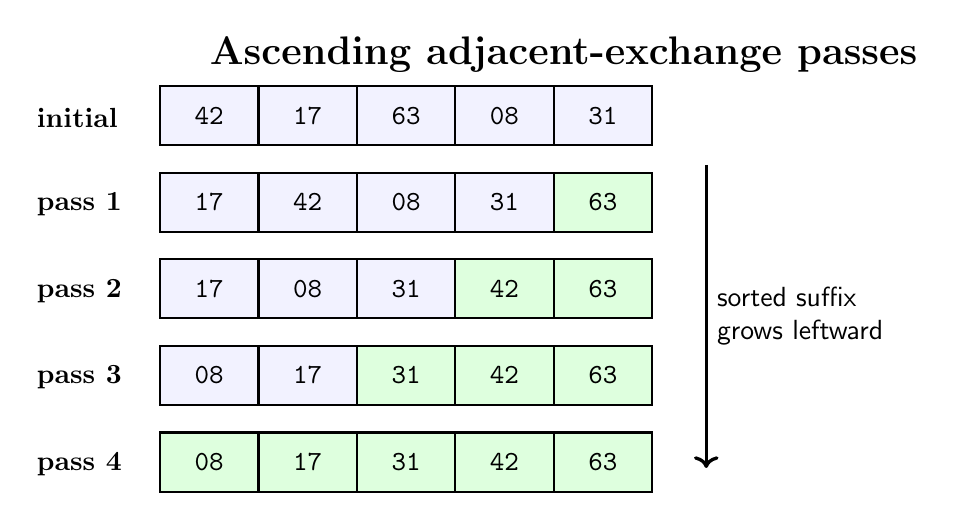
\begin{tikzpicture}[font=\sffamily,x=1.25cm,y=1.0cm]
\node[font=\Large\bfseries] at (4.1,6.15) {Ascending adjacent-exchange passes};
\foreach \y/\lab/\vals/\fixed in {
  5.0/initial/{42,17,63,08,31}/0,
  3.9/pass 1/{17,42,08,31,63}/1,
  2.8/pass 2/{17,08,31,42,63}/2,
  1.7/pass 3/{08,17,31,42,63}/3,
  .6/pass 4/{08,17,31,42,63}/5}{
  \node[right,font=\bfseries] at (-1.35,\y+.35) {\lab};
  \foreach \v [count=\i from 0] in \vals {
    \pgfmathtruncatemacro{\isfixed}{\i >= 5-\fixed ? 1 : 0}
    \ifnum\isfixed=1
      \fill[green!13] (\i,\y) rectangle ++(1,.75);
    \else
      \fill[blue!5] (\i,\y) rectangle ++(1,.75);
    \fi
    \draw[thick] (\i,\y) rectangle ++(1,.75);
    \node at (\i+.5,\y+.375) {\texttt{\v}};
  }
}
\draw[very thick,->] (5.55,4.75)--(5.55,.9) node[midway,right,align=left] {sorted suffix\\grows leftward};
\end{tikzpicture}
\end{document}
